\documentclass[twocolumn]{article}
\usepackage[utf8]{inputenc}
\usepackage[english]{babel}
\usepackage{lipsum}
\usepackage{multicol}
\usepackage{abstract} % Allows abstract customization
\usepackage{footnote}
\usepackage{listings}
\usepackage{url}
\usepackage{dblfnote}
\usepackage{graphicx}
\usepackage[margin=1in]{geometry}
\usepackage{cite}
\usepackage{natbib}
\usepackage{amsmath}
\usepackage{listings}
\usepackage{verbatim}
\newcommand{\code}[1]{\texttt{#1}}
\graphicspath{ {../images/} }
\bibliographystyle{acm} 
\setlength{\columnsep}{1cm}
\lstset{language=C}

\begin{document}

\twocolumn[\begin{@twocolumnfalse}
  \centerline{\Large\bfseries Breaking Petya - Solving a Poor Implementation of Salsa}
  \vspace{3ex}
  \centerline{Peixian Wang}
  \centerline{May 10, 2016}
  \vspace{3ex}
  
  \begin{abstract}
	  Ransomware has become a relatively profitable development in recent years with the surge in popularity of Bitcoin and other untracable forms of money transactions. In this paper we detail Petya, a recent form of ransomware targeting Windows platforms and NTFS drives. We describe the construction of Petya and the underlying encryption algorithm, Salsa20, and also present one possible solution called Infestor, which utilizes Z3, an efficient satisfiabliity modulo theory solver, to defeat Petya. 
  \end{abstract}
   \vspace{3ex}
\end{@twocolumnfalse}]

\section{Introduction}
\label{sec:introduction}
Online transactions through Tor \cite{tor} using anonomyous cryptocurrencies allow for a certain level of privacy when it comes to payments, but also allow themselves to be used in a malicious fashion. Since Bitcoin, the most popular form of cryptocurrency, makes it extremely hard to track the transactions, Bitcoin has become the de facto standard for ransomware, malware which infects the victim's computer, holds files hostage through encryption, and extorts the victims for money in return for the files. Petya is one such ransomware, except rather than targeting the files of the victim, it targets the master boot record (MBR) and master file table (MFT) \cite{decryptPetya}.

\section{Petya}
\label{sec:petya}
\subsection{Overview}
Petya is a relatively new ransomware variant, only starting to appear within the early months of 2016. In order to bypass the lengthy process of encrypting each file on the victim's hard drive, Petya simply seeks to write malicious code to the start of the disk. This code overwrites the MBR of the hard drive with a small kernel that then encrypts the MFT. 
\subsection{Behavioral Analysis}
\begin{figure}
	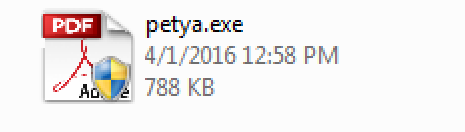
\includegraphics{petya.png}
	\caption{The petya executable disguised as a .pdf file.}
	\label{fig:petya}
\end{figure}
\begin{figure}
	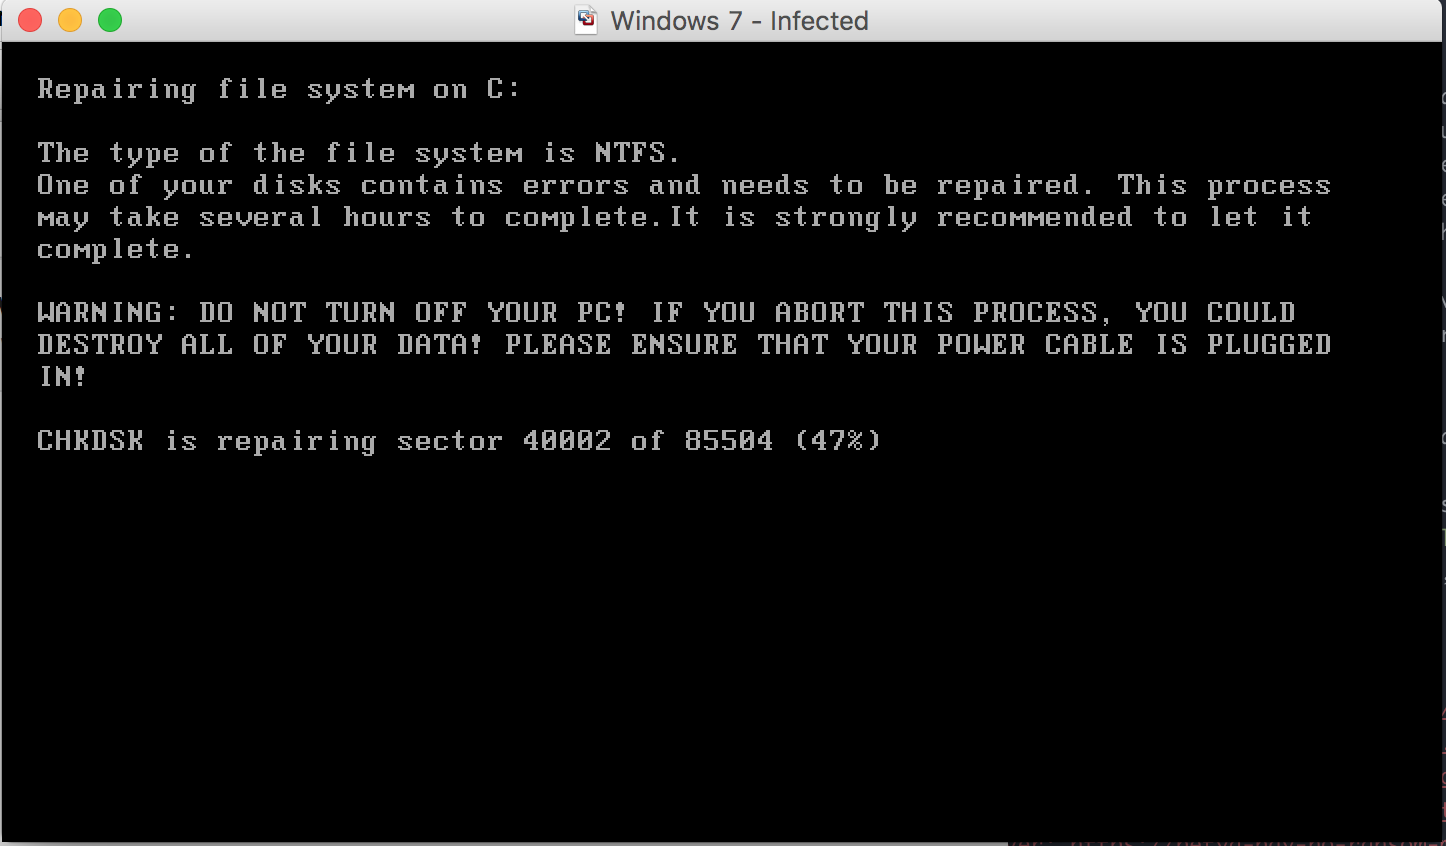
\includegraphics[width = 0.5\textwidth]{encryptionScreen.png}
	\caption{The fake CHKDSK scan made by Petya while it encrypts the MFT.}
	\label{fig:fakechk}
\end{figure}
\begin{figure}
	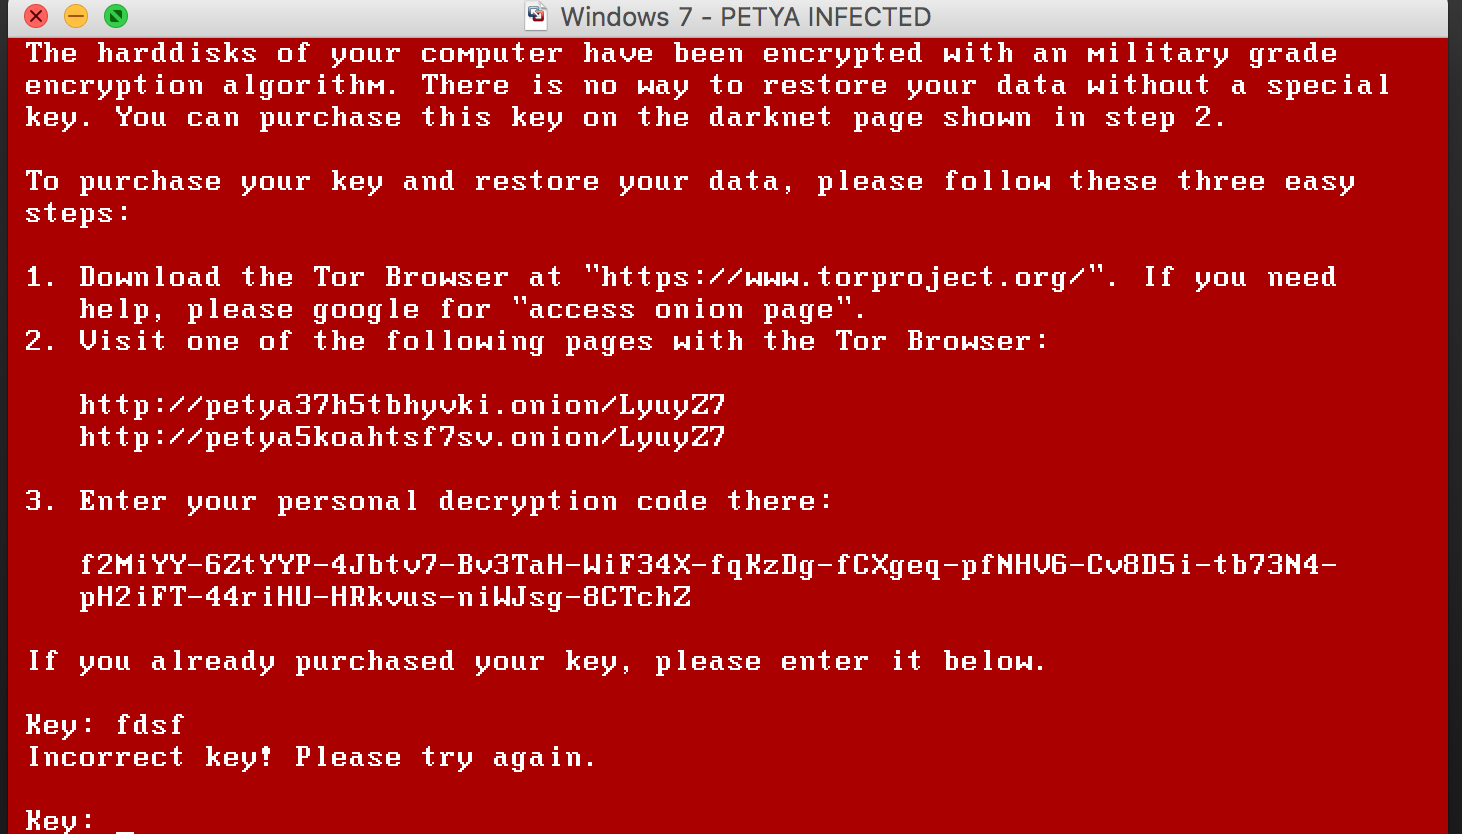
\includegraphics[width = 0.5\textwidth]{ransomScreen.png}
	\caption{The ransom note by Petya.}
	\label{fig:ransomScreen}
\end{figure}
\begin{figure}
	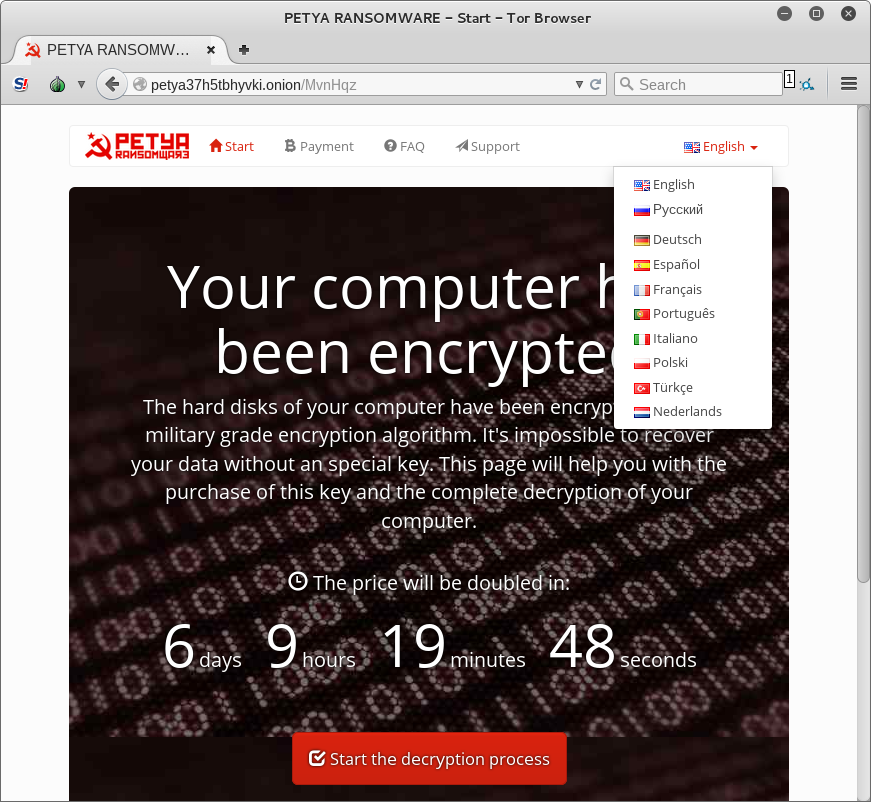
\includegraphics[width = 0.5\textwidth]{victimSite.png}
	\caption{Accessibility is important, even for malware. From \cite{lowLevelPetya}.}
	\label{fig:victimSite}
\end{figure}

Petya is usually destributed through a zip file \cite{lowLevelPetya}, containing two other files: 1. a photo of a young man, puporting to be an applicant and 2. an executable, disguised as a csv file, shown in figure \ref{fig:petya}. 
After opening the executable, Petya calls an undocumented API called \code{NtRaiseHardError}. The computer then promptly crashes and boots into a fake CHKDSK scan, shown in figure \ref{fig:fakechk}, which starts the encryption on the MFT. When the encryption completes, the user is shown a ransom note screen, shown in figure \ref{fig:ransomScreen}. After visiting the website, the user is presented with a relatively upscale website, featuring multiple languages (figure \ref{fig:victimSite}) and a tutorial on how victims can perform a bitcoin transaction (figure \ref{fig:victimTutorial}). 
\begin{figure}
	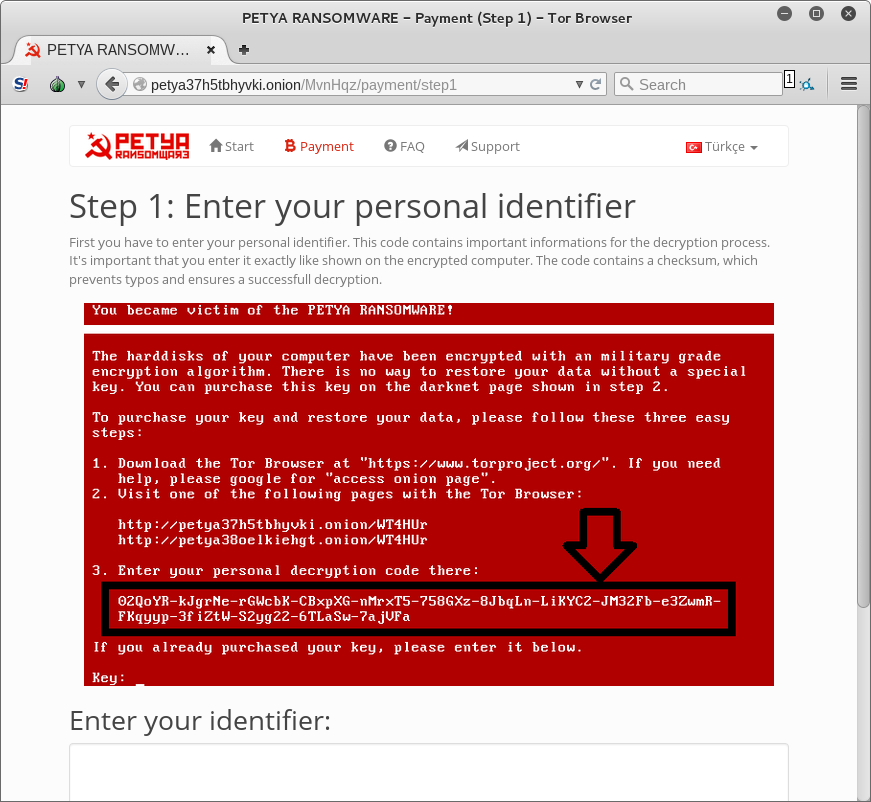
\includegraphics[width = 0.5\textwidth]{victimTutorial.png}
	\caption{Petya Tutorial on purchasing bitcoins and performing a transaction. From \cite{lowLevelPetya}.}
	\label{fig:victimTutorial}
\end{figure}

\subsection{Code Analysis}
The Petya attack can be detailed into 3 stages, the MBR attack stage, the MFT attack stage, and the ransom demand stage.
\subsubsection{Stage 0 - MBR attack}
In order to start analysis on Petya, the Windows executable must be examined. The executable generates a 8-byte initalization vector and a unique 16-byte random key that is used for further encryption, which also must be known to attackers to decrypt the files \cite{lowLevelPetya}. This key is expanded into the 32-byte encryption key using figure \ref{ls:key_expand}. Both of these values are used later on in the encryption process \cite{decryptPetya}. 

Petya then encrypts the original MBR by XOR'ing the contents of the MBR with \code{0x37} \cite{breakingPetya}. The encrypted value is then saved to sector 56 in the disk \cite{xrayPetya}. Disk sector 1-34 is encrypted in the same method. Petya then proceeds to write its own kernel, creating an \code{ONION\_SECTOR} structure and writing it to sector 54, shown in figure \ref{fig:onion_sector}. This data conviently contains 8 byte \code{iv}, which is the initalization vector required later on to decrypt. Sector 55 is then filled with the byte \code{0x37}, which is checked after the decryption process for validation purposes.

\begin{figure}
	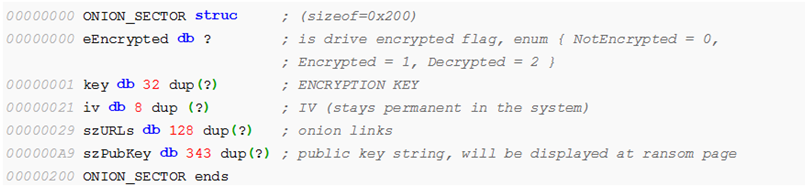
\includegraphics[width = 0.5\textwidth]{onion_sector.png}
	\caption{The \code{ONION\_SECTOR} struct, from \cite{decryptPetya}. }
	\label{fig:onion_sector}	
\end{figure}

\begin{figure*}
	\lstinputlisting[language=C]{petyaCode/key_expand.c}
	\caption{The key expansion method called by Petya. From \cite{decryptPetya}.}
	\label{ls:key_expand}
\end{figure*}

Finally, the \code{NtRaiseHardError} is called, crashing the victim's system. 

\subsubsection{Stage 1}
The system drive is queried by the Petya kernel, and upon returning a succesful value, Petya begins to overwrite the MFT while masquerading as a CHKDSK \cite{xrayPetya}. 

This stage can be devided into two steps: reading the key and deletion of the key, and encrypting sector 55. 

In the first step, Petya reads sector 54 into memory, which currently contains the \code{ONION\_SECTOR}. It copies the first 32 bytes of the \code{ONION\_SECTOR} into memory, which is the encryption key, and then proceeds to zero the first 32 bytes of data. Afterwards, the 32-byte key is only present in memory. 

The second step consists of Petya encrypting sector 55, which is currently filled will all byte values of \code{0x37}. Here Petya uses a flawed version of Salsa20 \cite{salsa20Spec}, passing in the 32-byte encryption key and the 8-byte initialization vector, to encrypt sector 55, which we will detail in section \ref{sec:salsa}.

\subsubsection{Stage 2}
Finally, Petya simply reboots into the red flashing skull screen, displaying the ransom note and providing an entry for the decryption key. By running the infected disk through a debugger, we can follow the verification process of the key:

\begin{enumerate}
	\item Read sector 54 to read the 8 byte intialization vector.
	\item Read sector 55.
	\item Read the user entered key, extract the first 16 bytes, and use the same expansion function as \ref{ls:key_expand} in order to retrieve a 32-byte key.
	\item Use the 32 byte key and the 8 byte initialization vector to decrypt sector 55, if all the values equal \code{0x37}, then the user entered key is correct. Else throw an \code{Invalid Key!}.
	\item If the user entered key is correct, proceed with the decryption process and ask user to restart their computer. 
\end{enumerate}

From this verification process, we can begin to construct a list of constraints the key must follow:

\begin{enumerate}
	\item Only the first 16 bytes are extracted from the user entry, meaning the key must be at most 16 bytes long from the character set \verb|[a-zA-Z0-9]|, i.e. all alphanumerical characters.
	\item The key must enable all data in sector 55 to be able to xor with \code{0x37}.
	\item The initialization vector must be used shuffled in somehow.  
\end{enumerate}

Thus, in order to break Petya, we must start by breaking its encryption algorithm: Salsa.

\section{Salsa}
\label{sec:salsa}
\subsection{Salsa20 Spec}
Salsa20, at its core, is a function that takes a 64-byte string and produces a 64-byte string. The function follows an add-rotate-xor operation, whose operation can be found in exact detail in the Salsa20 spec \cite{salsa20Spec}, but the original implementation uses a 32-byte encryption key and an 8-byte initilization vector to produce a final 515-bit key-stream, shown in figure \ref{fig:salsaChart}. 

To create the output, the 64 byte input into Salsa is seen in little-endian form as 16 words, which are fed into 320 invertible modifications, where each modification changes one words. The resulting 16 words are added to the orginal input respectively mod $2^32$, which then produces the output in little-endian form. The exact modification is predefined in the Salsa spec and implementations \cite{salsa20}, which is a series of 10 identical double-rounds, each consisting of 4 parallel quarter-rounds, with each quarter-round modifying 4 words \cite{salsa20Core}. 


\begin{figure*}
	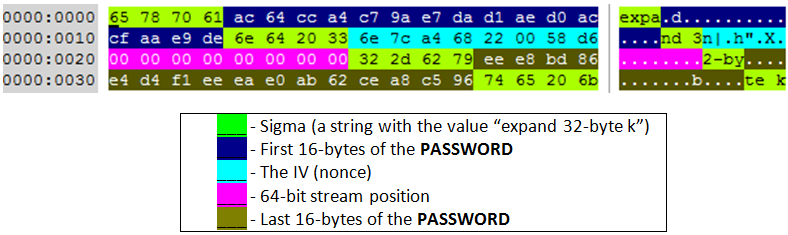
\includegraphics[width = \textwidth]{salsaChart.png}
	\caption{The original Salsa implementation. From \cite{decryptPetya}.}
	\label{fig:salsaChart}
\end{figure*}

\section{Infestor}
\label{sec:infestor}
\subsection{Code Walkthrough}

\bibliography{paper} 

\end{document}